\chapter{Classification à l'aide de l'algorithme K plus proches voisins (KNN)}
	\section{Introduction}
		\paragraph{}
		Un des principaux problème auquel nous devons faire face quand nous exploitant des données réelles est l'inférence d'une étiquette pour une nouvelle donnée non rencontrée avant, c'est la définition d'un problème de classification, et il a beaucoup de domaine d'application (détection de fraude, détection d'intrusion, évaluation de la qualité d'un produit ...). L'un des nombreux algorithmes mis au point pour résoudre ce type de problème est l'algorithme des K plus proches voisins ou K-Nearest-Neighbors (KNN).
		\par 
		 L'algorithme est basé sur une mesure de similarité appelé \textbf{Distance} dans un voisinage suivit de l'attribution d'une étiquette sur la base d'un vote a majorité (pondéré ou pas) des représentant du voisinage en question, l'étiquette est donc attribué selon la similarité entre un point (une instance) et ce voisinage.
	\newpage
	\section{Définitions}
		\paragraph{}
		Avant de détailler le fonctionnement de l'algorithme nous allons introduire quelques notions pour mieux comprendre son fonctionnement
		\subsection{Point}
			\paragraph{}
			Un point $P$ est une instance du dataset, c.à.d un ensemble $P_att$ de valeur d'attributs, plus formellement, un point est est l'extrémité d'un vecteur : \[\vec{V} = a_1.\vec{v_1} + a_2.\vec{v_2} + ... + a_n.\vec{v_n} \]
			où : 
			\begin{itemize}
				\item $\vec{v_i} $ : est un vecteur unité de base ( vecteur caractéristique d'un attribut )
				\item $n$ : le nombre d'attribut d'un point donné
			\end{itemize}
		Le point dont nous parlons est donc analogue à un point dans un espace multi-dimensionnel désigné par des coordonnées cartésiennes.
		\subsection{Distance}\label{distance}
			\paragraph{}
			La notion de distance est une valeur (très souvent numérique) qui quantifie la mesure de similarité entre deux point dans une espace multi-dimensionnel, la distance tendra donc à être de plus en plus petite si deux points sont très similaires, et inversement elle sera de plus en plus grande si ces deux points sont de plus en plus différents.
			\par
			Il existe plusieurs façon de mesurer la distance entre deux points donnée dans une espace multi-dimensionnel, nous avons choisi pour cela d'utiliser la distance d'ordre 2 (2-distance) plus connue sous le nom de distance euclidienne dont la formule est la suivante : 
			\begin{gather*} 
				\text{Soient deux points } X(x_1,...,x_n) \text{ et } Y(y_1,...,y_n) \\
				\text{Et soit la distance }D_p(X,Y) = \sqrt[p]{\sum_{i=1}^{n} | x_i - y_i|^p} \\
				\text{La distance euclidienen 2-distance est la suivante : } \\
				D_2(X,Y) = \sqrt{\sum_{i=1}^{n} (x_i - y_i)^2} \\
			\end{gather*}
			\par
			Il reste donc à définir la sémantique de l'opérateur $-$ qui lui introduit la distance élémentaire entre deux valeur d'un même attribut, dans le cas numérique cette opérateur est l'opérateur arithmétique classique de la soustraction, pour les valeurs nominales nous avons choisis une interprétation simple pour faciliter l'exploitation de l'algorithme par la suite qui est la suivante : 
			\[ 
				x_{nom} - y_{nom} = 
				\begin{cases}
					1 & \quad\text{ Si } x_{nom} = y_{nom}\\
					0 & \quad\text{ Sinon }
				\end{cases}
			\] 
			\par Elle représente la distance de Hamming simplifiée au cas d'une variable a valeur binaires seulement.
		\subsection{Voisinage}
			\paragraph{}
			Le concept de voisinage d'un certain point $P$ est une notion très importante en classification et clustering, elle désigne l'ensemble de points $V$ qui sont similaires à un certain degré à $P$, plus particulièrement si $\forall v \in V$ on à $D_p(P,v)=minDst$ où $minDst$ est la plus petite distance entre deux points, alors $V$ est l'ensemble des voisins directes de $P$.
		\subsection{Classification}
			\paragraph{}
			Da manière informelle, étant donnée un ensemble d'instances (points) dont nous connaissons l'étiquette (ou la classe), la classification est l'opération d'affectation d'une classe à une nouvelle instance qui n'a pas encore été classifié avant.
			Ainsi un algorithme de classification est une fonction $F$ telle qu'étant donné un ensemble de points $E$ et un ensemble de classes $C$ : 
			\begin{gather*}
				F : E \rightarrow C \\
				F(p \in E) = c 
			\end{gather*}
		\subsection{Précision}
			\paragraph{}
			Pour un classifier $F$, nous somme souvent amené a mesurer son degré d'exactitude sur un ensemble de test, la précision est une mesure qui reste naïve mais donne une bonne approximation de la qualité de la classification, elle consiste en un rapport entre le nombre de classes correctement prédites sur le nombre total des instances à classifier dans l'ensemble de test.
			Plus formellement : 
			\begin{gather*}
				\text{Soient } \hat{F} \text{  une fonction qui donne toujours la classe exacte à un instance} \\
				\text{Et } T={(Att,C)} \text{  Un ensemble de paires Attributs et Classe} \\
				\text{Et } Pred =\lbrace t \in T | F(t) = \hat{F}(t) \rbrace \text{  L'ensemble des points dont la prediction est correcte} \\
				\text{Alors la précision par rapport au classifier F est :  } \\
				P_F = \frac{|Pred|}{|T|}	
			\end{gather*}
	\section{Algorithme}
		\paragraph{}
		L'algorithme \textbf{KNN} se base comme cité précédemment sur le principe du vote majoritaire, en effet si un individu est proche d'un ensemble d'autre individus qui lui sont similaires, ses caractéristiques seront elles aussi similaires aux individus dont l'étiquette est la plus dominante (cette façon de penser peut introduire la notion de bruit ou valeurs déviantes que nous verrons par la suite).
		\par L'algorithme dispose d'un paramètre empirique :
		\begin{itemize}
			\item \textbf{K} : le nombre de voisins à analyser pour un point donnée
		\end{itemize}
		Mais il dépend aussi de la taille et la diversité de l'échantillon d'apprentissage en entrée. Le choix du paramètre K est une étape cruciale qui déterminera les performance de l'algorithme, pour faciliter l'étape de classification (après le vote de la majorité) on prendra un $K = 2*m+1$ avec $m \in \mathbb{N}$ qui sera donc impair pour qu'une majorité émerge, cependant cette restriction ne règle le problème que si $K > |C|$ où $|C|$ est le nombre de classes, en effet si l'on observe que $K$ voisins dans le cas où $K \leq |C|$, il y aura toujours une chance que les voisins soient tous étiquetés avec une classe $c \in C$ différentes pour chacun. 
		
		\par 
		Le pseudo-code suivant détaille les étapes à suivre : 
		
		\begin{algorithm}[H]
			\caption{KNN}
			\SetKwInOut{Input}{Entrée}\SetKwInOut{Output}{Sortie}
			\SetKwFunction{sort}{TrierParPlusPetiteDistance}
			\SetKwFunction{cls}{ClasseDominante}
			
			\Input{(E : Ensemble des instances d'apprentissage, X : instance à classifier , K : entier)}
			\Output{(C : Classe inférée de X )}
			\textbf{Var :} \\
			$Distances : \text{ Ensemble des paires (point,D(X,point))}$ ;\\
			$Distances \gets \emptyset $;\\
			\For{$e \in E$}
			{
				$Distances \gets Distances \bigcup \lbrace (e,D_2(X,e)) \rbrace$ ;\\
			}
			
			$Distances\_tri \gets $ \sort{$Distances$};\\
			$D_K \gets \lbrace D_i \in Distances\_tri | i = 1..K\rbrace$;\\
			$C \gets $ \cls{$D_K$};\\
			\KwRet{$C$}
		\end{algorithm}
		
		
	\section{Implémentation}
		\paragraph{}
		Pour mieux visualiser la structure interne de notre implémentation, nous allons présenter d'abord un diagramme \textbf{UML} puis ensuite détailler les composants du module \textbf{KNN} : 
		\begin{figure}[H]
			\centering
			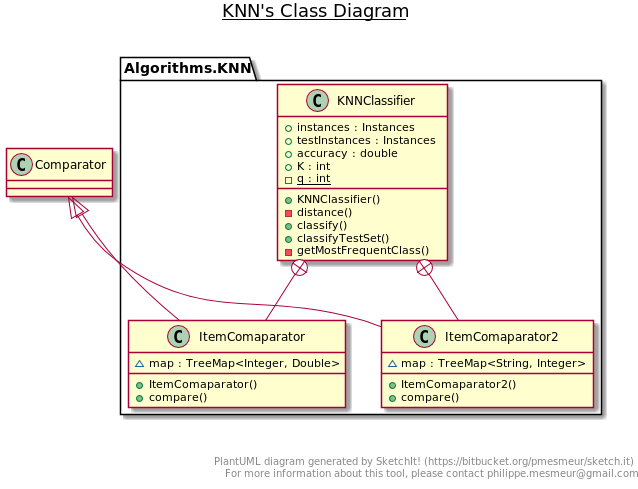
\includegraphics[width=0.75\linewidth]{knn/images/uml.png}
		\end{figure}
		Le module est composé de deux parties majeures : 
		\begin{itemize}
			\item Deux classes \textbf{ItemComparator} et \textbf{ItemComparator2} qui implémentent chacune la fonction \textbf{compare} de l'interface \textbf{Comparator}, cela est dû au fait que nous avons eu besoin de trier deux structures de hachage de la classe \textbf{TreeMap} selon les \textbf{valeurs} dans l'ordre croissant et décroissant.
			
			\item La classe \textbf{KNNClassifier} qui contiendra les méthodes et attributs nécessaire pour l'exécution de l'algorithme. 
		\end{itemize}
		\subsection{KNNClassifier} 
		Il est maintenant temps de détailler le contenu de la classe \textbf{KNNClassifier} : 
		\begin{itemize}
			\item Les attributs sont les suivants : 
			\begin{figure}[H]
				\centering
				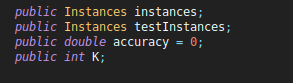
\includegraphics[width=0.75\linewidth]{knn/images/props.png}
			\end{figure}
			\par 
			Les deux premiers sont des objets de la classe \textbf{weka.Instances}, ils représentent respectivement les échantillons d'apprentissage et de test. Ensuite nous avons défini les deux paramètre de notre algorithme \textbf{K} le nombre de voisins à tester et \textbf{ratio} le taux de division entre échantillons d'apprentissage et de test. Ici \textbf{q} le paramètre de distance \textbf{p} vu dans \ref{distance}
			
			
			\item Les méthodes implémentées sont les suivantes : 
				\begin{figure}[H]
				\centering
				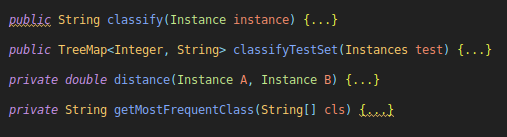
\includegraphics[width=0.75\linewidth]{knn/images/meths.png}
			\end{figure}
			\begin{itemize}
				\item \textbf{classify} c'est la méthode principale qui prend une instance en entrée et retourne sa classe prédite en sortie.
				\item \textbf{classifyTestSet} c'est une méthode qui fait appel à \textbf{classify} sur un ensemble de test dont les classes sont connues, et calcule la précision de la classification effectuée
				\item la méthode de calcul d'une distance \ref{distance} entre deux points ( instances ) données
				\item \textbf{getMostFrequentClass} elle extrait d'un ensemble de classes, celle qui est la plus fréquente en terme d'apparition.
			\end{itemize}
		\end{itemize}
	\section{Interface graphique}
		\paragraph{}
		De manière équivalente à ce que nous avons fait pour le module précédent (\ref{apriori}) Nous avons intégré à l'interface graphique principale l'algorithme \textbf{KNN}, voici l'interface choisie suivit de quelques explications : 
		\begin{figure}[H]
			\centering
			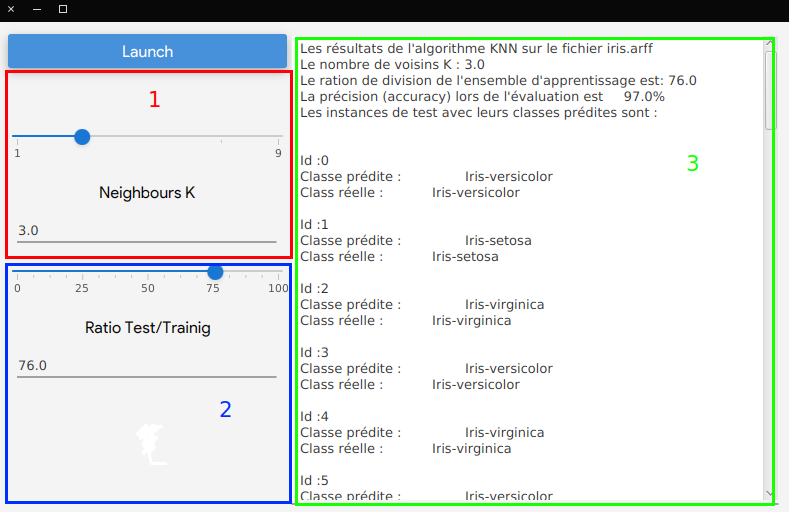
\includegraphics[width=0.75\linewidth]{knn/images/app.png}
		\end{figure}
		\paragraph{}
		L'interface se compose de 3 zones :
		\begin{itemize}
			\item \textbf{Zone 1 et 2:} permettre d'introduire les valeurs des hyper paramètres (K et ratio)
			\item \textbf{Zone 3:} affichage du résultat comme une liste d'instances avec leurs classes prédites et leurs classes réelles, ainsi que la précision de la classification. 
		\end{itemize}
	
	\section{Résultats expérimentaux}
		\subsection{Choix du dataset}
			\paragraph{}
			Puisque nous disposons d'un moyen de calculer une distance entre deux points dont les attributs sont soit nominaux soit numériques, nous avons choisis de tester les 3 combinaisons de ces choix, c.à.d : 
			\begin{itemize}
				\item Dataset purement numérique : nous avons choisis le dataset \textbf{iris.arff}
				\item Dataset purement nominal : nous avons choisis le dataset \textbf{car.arff}
				\item Dataset hybride nous avons choisis le dataset \textbf{credit-g.arff}
			\end{itemize}
			\par la taille des datasets est un critère important à prendre en compte, plus la taille est grande plus le temps d'inférence (étiquetage d'une nouvelle instance) pourrait être grand, car il faudra donc parcourir toutes les instances dans l'échantillon d'apprentissage, néanmoins, si nous posons $N$ comme le nombre de ces instances, et $K$ le nombre d'attributs pour chaque instances, il faudra donc parcourir les $K$ attributs de chacune des $N$ instances puis insérer la distances $D$ dans une structure de hachage en $O(log(M))$ où $M$ est le nombre de voisins, ce qui nous donne donc une complexité temporelle $O(N*K*Log(M))$ ce qui reste assez raisonnable a plus grande échelle.
		\subsubsection{Variations des paramètres}
			\paragraph{}
			Pour ce qui est des paramètres, nous avons décidé de faire varier le nombre de voisins $K$ ans l'intervalle $\left[ \text{3 , 2*\textbf{NombreDeClasses}+1}\right]$ avec un pas $step = 2$ (pour s'assurer que les valeurs restent impairs).
			\par 
			Le paramètre \textbf{ratio} sera lui varié dans l'intervalle $\left[ 0.1 ,0.9 \right]$ (ce qui représente la taille de l'échantillon d'apprentissage)
		\subsection{Résultats}
			\paragraph{}
				Nous avons lancé l'algorithme sur les datasets mentionnés plus haut en gardant à chaque fois les informations nécessaires pour comparer les résultats (précision, temps d'exécution), les tableaux comparatifs suivants résument le processus, ils serons ensuite accompagnés de quelques commentaires :
				
			\subsubsection*{Résultats pour car.arff }
			\begin{table}[H]
				\centering
				\begin{tabular}{|c|c|c|c|c|c|}
					\hline
					\textbf{K} & \textbf{\begin{tabular}[c]{@{}c@{}}Nb instances\\  apprentissage\end{tabular}} & \textbf{\begin{tabular}[c]{@{}c@{}}Nb instances \\ test\end{tabular}} & \textbf{Précision} & \textbf{ratio} & \textbf{temps(s)} \\ \hline
					3          & 172,8                                                                          & 1555,2                                                                & 0,89               & 0,1            & 4,686             \\
					3          & 345,6                                                                          & 1382,4                                                                & 0,88               & 0,2            & 3,395             \\
					3          & 518,4                                                                          & 1209,6                                                                & 0,9                & 0,3            & 2,729             \\
					3          & 691,2                                                                          & 1036,8                                                                & 0,89               & 0,4            & 2,44              \\
					3          & 864                                                                            & 864                                                                   & 0,89               & 0,5            & 1,976             \\
					3          & 1036,8                                                                         & 691,2                                                                 & 0,9                & 0,6            & 1,556             \\
					3          & 1209,6                                                                         & 518,4                                                                 & 0,89               & 0,7            & 1,201             \\
					3          & 1382,4                                                                         & 345,6                                                                 & 0,89               & 0,8            & 0,816             \\
					3          & 1555,2                                                                         & 172,8                                                                 & 0,93               & 0,9            & 0,4               \\
					5          & 172,8                                                                          & 1555,2                                                                & 0,79               & 0,1            & 3,575             \\
					5          & 345,6                                                                          & 1382,4                                                                & 0,82               & 0,2            & 3,181             \\
					5          & 518,4                                                                          & 1209,6                                                                & 0,75               & 0,3            & 2,859             \\
					5          & 691,2                                                                          & 1036,8                                                                & 0,86               & 0,4            & 2,367             \\
					5          & 864                                                                            & 864                                                                   & 0,83               & 0,5            & 1,993             \\
					5          & 1036,8                                                                         & 691,2                                                                 & 0,83               & 0,6            & 1,605             \\
					5          & 1209,6                                                                         & 518,4                                                                 & 0,83               & 0,7            & 1,172             \\
					5          & 1382,4                                                                         & 345,6                                                                 & 0,8                & 0,8            & 0,792             \\
					5          & 1555,2                                                                         & 172,8                                                                 & 0,85               & 0,9            & 0,412             \\
					7          & 172,8                                                                          & 1555,2                                                                & 0,73               & 0,1            & 4,242             \\
					7          & 345,6                                                                          & 1382,4                                                                & 0,74               & 0,2            & 3,125             \\
					7          & 518,4                                                                          & 1209,6                                                                & 0,7                & 0,3            & 2,759             \\
					7          & 691,2                                                                          & 1036,8                                                                & 0,76               & 0,4            & 2,376             \\
					7          & 864                                                                            & 864                                                                   & 0,78               & 0,5            & 1,986             \\
					7          & 1036,8                                                                         & 691,2                                                                 & 0,83               & 0,6            & 1,581             \\
					7          & 1209,6                                                                         & 518,4                                                                 & 0,84               & 0,7            & 1,384             \\
					7          & 1382,4                                                                         & 345,6                                                                 & 0,83               & 0,8            & 0,791             \\
					7          & 1555,2                                                                         & 172,8                                                                 & 0,75               & 0,9            & 0,396             \\ \hline
				\end{tabular}
				\caption{Résultats de l'algorithme KNN sur le dataset car.arff}
			\end{table}
		\paragraph{}
		 Pour mieux visualiser les résultats, nous avons décidé de fixer un des paramètres ($K$) en faisant varier l'autre pour analyser en quoi ces variations pourraient affecter la précision de l'algorithme: 
		 \begin{figure}[H]
		 	\centering
		 	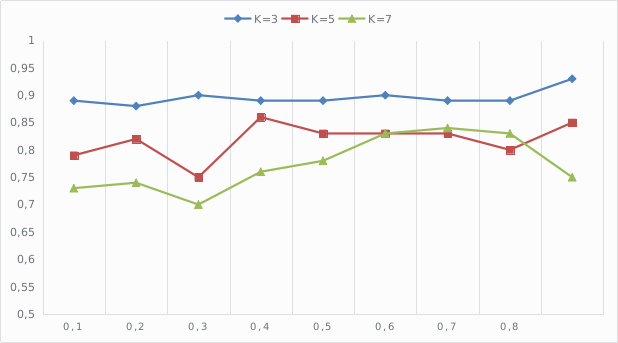
\includegraphics[width=0.75\linewidth]{knn/images/graph_car.png}
		 	\caption{Graphes comparatif des résultats de l'algorithme sur le dataset car.arff}
		 \end{figure}
	 	\paragraph{Commentaires}
	 		Du point de vue intrinsèque au choix de $K$ c.à.d si l'on ne compare pas entre les résultats de deux variations de ce paramètres différentes, on peut noter que le changement du ration d'apprentissage/test n'affecte pas beaucoup sur la précision, mise à part dans le cas où l'on choisi un trop gros échantillons d'apprentissage ce qui va biaiser le résultat final, auquel cas le classifier aura déjà une grande connaissance sur le dataset et la classification sera plus aisée.
	 		\par
	 		D'un point de vue extrinsèque aux choix de $K$, c.à.d si on compare la précision par rapport aux choix de ce dernier, il est a noté qu'un plus petit choix de ce paramètre donne systématiquement une meilleure précision avec de petites fluctuations (ceci n'est pas une règle générale, juste une observation sur notre jeu de tests). 
	 	
		\subsubsection*{Résultats pour iris.arff}
			\begin{table}[H]
				\centering
				\begin{tabular}{|c|c|c|c|c|c|}
					\hline
					\textbf{K} & \textbf{\begin{tabular}[c]{@{}c@{}}Nb instances \\ apprentissage\end{tabular}} & \textbf{\begin{tabular}[c]{@{}c@{}}Nb instances \\ test\end{tabular}} & \textbf{Précision} & \textbf{ratio} & \textbf{temps(s)} \\ \hline
					3          & 15                                                                             & 135                                                                   & 0,97               & 0,1            & 0,088          \\
					3          & 30                                                                             & 120                                                                   & 0,96               & 0,2            & 0,061          \\
					3          & 45                                                                             & 105                                                                   & 0,95               & 0,3            & 0,017          \\
					3          & 60                                                                             & 90                                                                    & 0,96               & 0,4            & 0,016          \\
					3          & 75                                                                             & 75                                                                    & 0,94               & 0,5            & 0,01           \\
					3          & 90                                                                             & 60                                                                    & 0,98               & 0,6            & 0,008          \\
					3          & 105                                                                            & 45                                                                    & 1                  & 0,7            & 0,008          \\
					3          & 120                                                                            & 30                                                                    & 1                  & 0,8            & 0,005          \\
					3          & 135                                                                            & 15                                                                    & 1                  & 0,9            & 0,003          \\
					5          & 15                                                                             & 135                                                                   & 0,96               & 0,1            & 0,023          \\
					5          & 30                                                                             & 120                                                                   & 0,95               & 0,2            & 0,019          \\
					5          & 45                                                                             & 105                                                                   & 0,97               & 0,3            & 0,02           \\
					5          & 60                                                                             & 90                                                                    & 0,96               & 0,4            & 0,017          \\
					5          & 75                                                                             & 75                                                                    & 0,96               & 0,5            & 0,012          \\
					5          & 90                                                                             & 60                                                                    & 0,95               & 0,6            & 0,011          \\
					5          & 105                                                                            & 45                                                                    & 1                  & 0,7            & 0,008          \\
					5          & 120                                                                            & 30                                                                    & 0,96               & 0,8            & 0,005          \\
					5          & 135                                                                            & 15                                                                    & 0,93               & 0,9            & 0,003          \\ \hline
				\end{tabular}
				\caption{Résultat de l'algorithme KNN sur iris.arff}
				\label{my-label}
			\end{table}
		\begin{figure}[H]
			\centering
			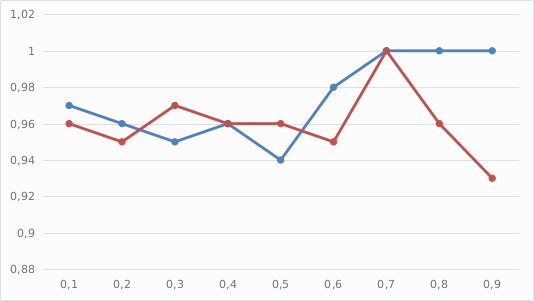
\includegraphics[width=0.75\linewidth]{knn/images/graph_iris.png}
			\caption{Graphes comparatif des résultats de l'algorithme sur le dataset iris.arff}
		\end{figure}
		\paragraph{Commentaires : }
		Pour ce dataset, contrairement au précédent, du point de vue intrinsèque au choix de $K$, il n'est pas garantie que la précision augmente si le taux d'apprentissage augmente, on peut le voir pour la courbe en \textcolor{red}{rouge} où la précision a diminué, certe d'un petit pas (de l'ordre de 0.08), mais à plus grande échelle cette quantité deviendrait cruciale. 
		\par Il est aussi a noté que la classification est assez rapide pour des valeurs numériques.
		
	\subsubsection{Résultats pour credit-g.arff}
		\begin{table}[H]
			\centering
			\begin{tabular}{|c|c|c|c|c|c|}
				\hline
				\textbf{K} & \textbf{Nb instances apprentissage} & \textbf{Nb instances test} & \textbf{Précision} & \textbf{ratio} & \textbf{temps} \\ \hline
				3          & 100                                 & 900                        & 0,85               & 0,1            & 3,982          \\
				3          & 200                                 & 800                        & 0,85               & 0,2            & 4,066          \\
				3          & 300                                 & 700                        & 0,87               & 0,3            & 3,132          \\
				3          & 400                                 & 600                        & 0,86               & 0,4            & 2,632          \\
				3          & 500                                 & 500                        & 0,86               & 0,5            & 2,289          \\
				3          & 600                                 & 400                        & 0,86               & 0,6            & 1,791          \\
				3          & 700                                 & 300                        & 0,87               & 0,7            & 1,321          \\
				3          & 800                                 & 200                        & 0,86               & 0,8            & 0,886          \\
				3          & 900                                 & 100                        & 0,83               & 0,9            & 0,446          \\ \hline
			\end{tabular}
			\caption{Résultats de l'algorithme KNN sur le dataset credit-g.arff}
			\label{my-label}
		\end{table}
		\begin{figure}[H]
			\centering
			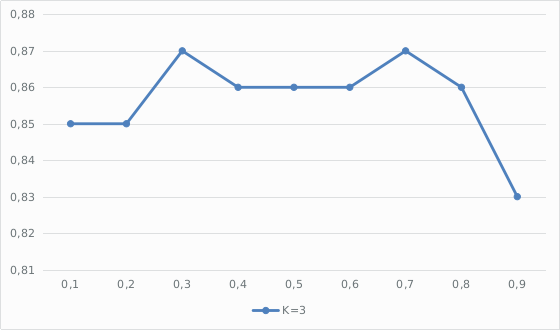
\includegraphics[width=0.75\linewidth]{knn/images/graph_credit.png}
			\caption{Graphes comparatif des résultats de l'algorithme sur le dataset credit-g.arff}
		\end{figure}
		\paragraph{Commentaires : }
		De manière analogue au dataset précédent, du point de vue intrinsèque au choix de $K$, laa précision peu diminuer dans le cas où le taux d'apprentissage augmente, on peut le voir pour la courbe en \textcolor{blue}{bleu} où la précision a diminué d'un facteur de 0.04
		\par Il est aussi a noté que la classification à pris un temps assez considérable pour(peut être du à la présence d'attributs nominales ? )
	\section{Conclusion}
